\documentclass[../tufte-style.tex]{standalone}

\begin{document}

\date{March 2, 2026}


\begin{frame}{Critical Points}

    \begin{block}{What are the critical points?}
        Critical points are the roots of the derivative of a funciton or the values of the domain in which the derivative is undefined.
    \end{block}

    \hfill

    \begin{block}{Why we are interested in critical points?}
        Critical points are essential for identifying potential local maxima, minima, or inflection points in the graph of the function. 
    \end{block}


\end{frame}

\begin{frame}{Example: \(f(x) = e^{\cos(x)}\)}

The derivative of the function \(f(x) = e^{\cos(x)}\), by using the chain rule, is 
\begin{gather*}
    f'(x) = -e^{\cos(x)}\sin(x).
\end{gather*}
Then to compute find the critical points we need to equate the derivative to zero and solve for \(x\),
\begin{gather*}
    f'(x) = 0 \leftrightarrow -e^{\cos(x)}\sin(x) = 0
\end{gather*}

\end{frame}

\begin{frame}{Example: \(f(x) = e^{\cos(x)}\)}

To solve \(-e^{\cos(x)}\sin(x) = 0\)
we have two possible solutions:
\begin{gather*}
e^{\cos(x)} = 0,\quad \sin(x) = 0
\end{gather*}

\begin{minipage}[c]{0.45\textwidth}
\begin{block}{\(\sin(x)=0\)}
    The solutions of this equation are,
    \begin{gather*}
        x= n\pi,~n\in\mathbb{Z}
    \end{gather*}
\end{block}
\end{minipage}
\hfill
\begin{minipage}[c]{0.45\textwidth}
\begin{block}{\(e^{\cos(x)}=0\)}
    \begin{align*}
        \cos(x) &= \ln(0)
    \end{align*}
    \centering
    No solution.
\end{block}
\end{minipage}

\end{frame}


\begin{frame}{Example: \(f(x) = e^{\cos(x)}\)}

Since we have only solution for \(\sin(x)=0\) the critical points of the function \(f(x)\) are,
\begin{empheq}[box=\tcbhighmath]{equation*}
    x= n\pi,~n\in\mathbb{Z}
\end{empheq}

\end{frame}

\begin{frame}{Example: \(f(x) = e^{\cos(x)}\)}

\begin{figure}[ht!]
    \centering
    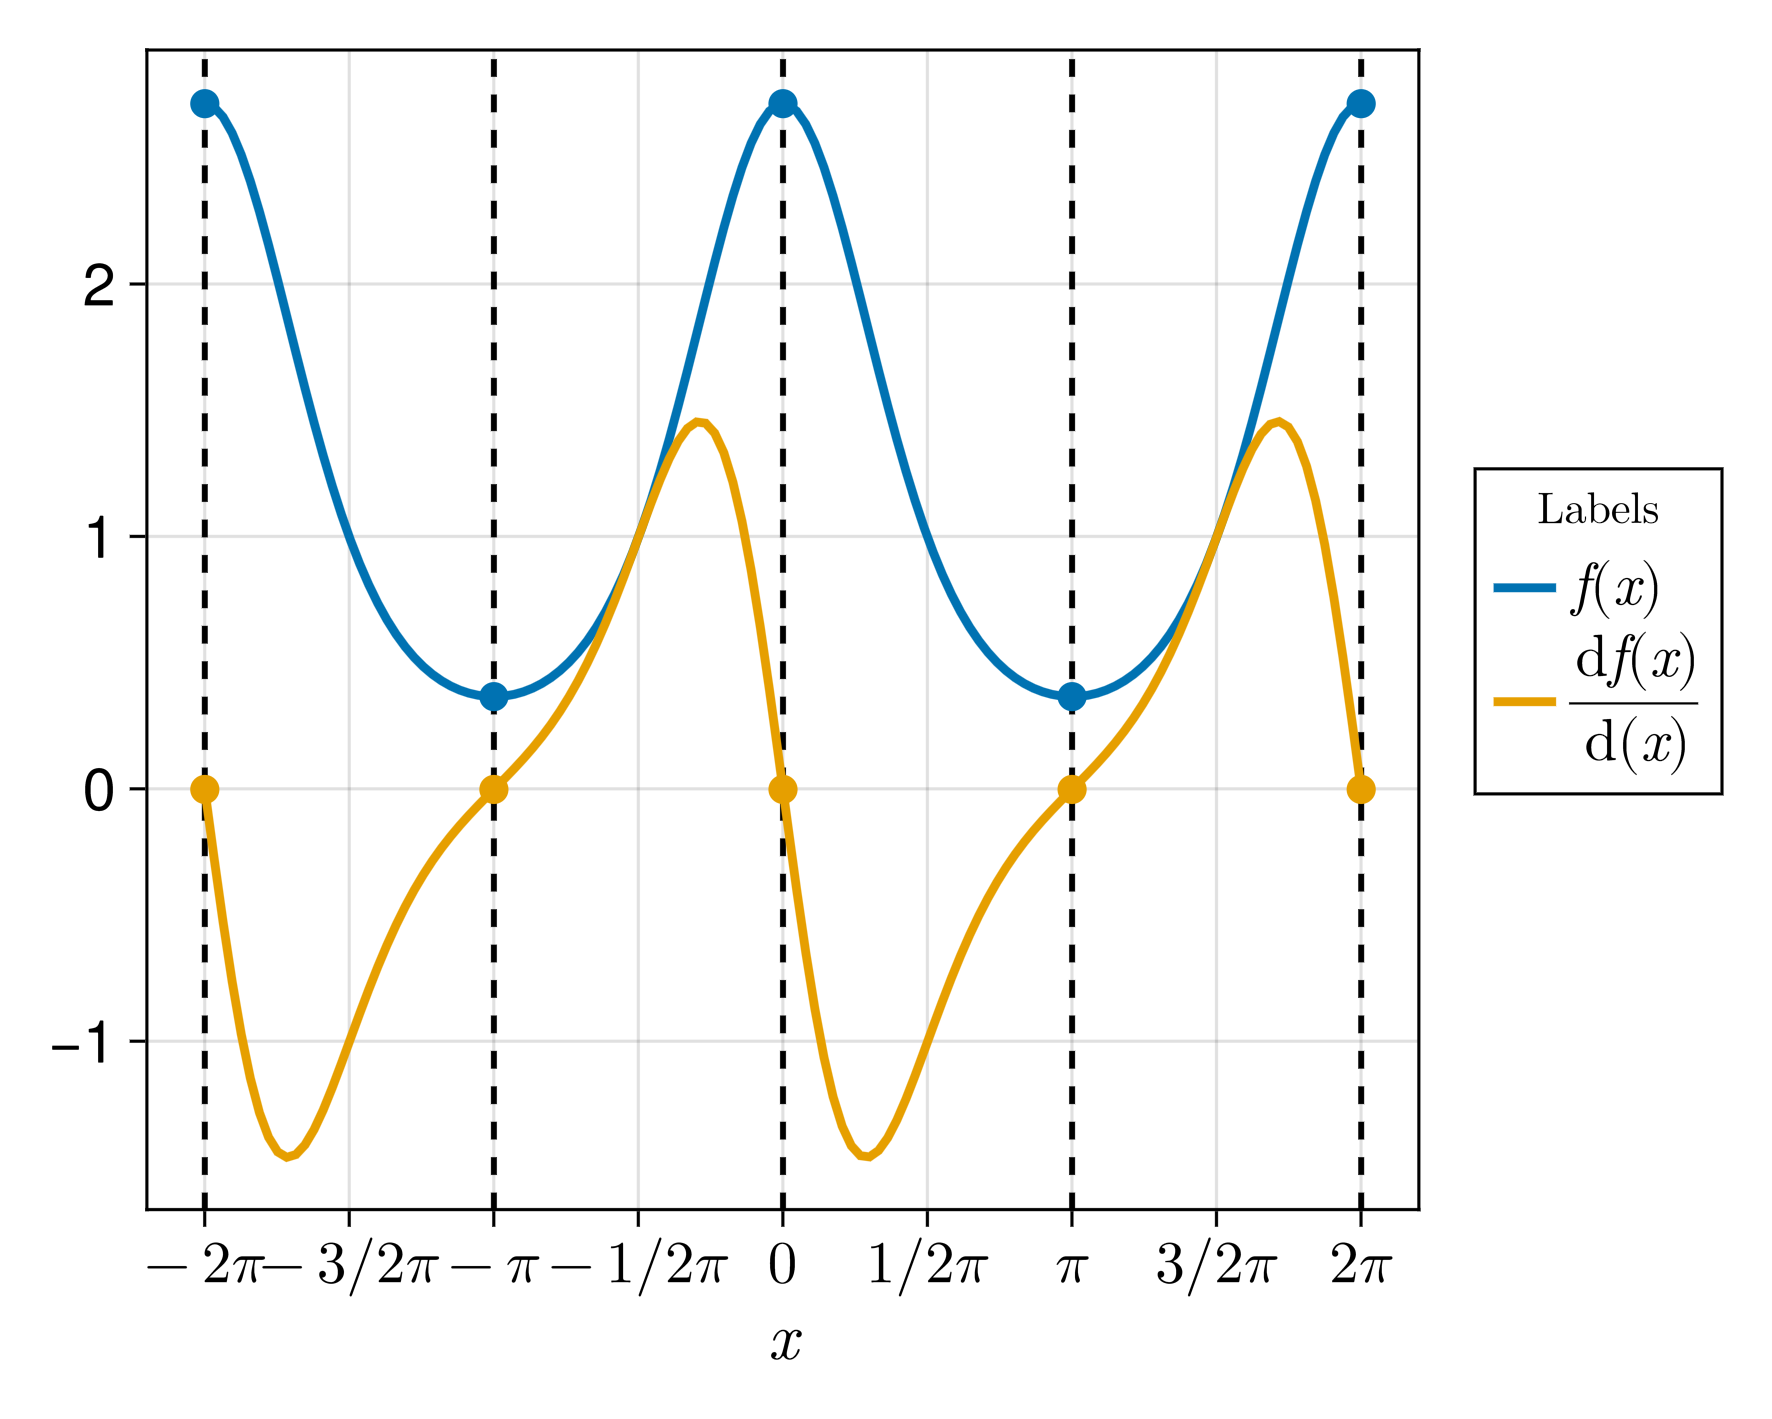
\includegraphics[width=0.6\textwidth]{../Figures/fig_e(cos(x)).png}
\end{figure}

\end{frame}

\begin{frame}{Class activity}

Compute the derivative of the following function.
Then find its critical point.

\begin{gather*}
    P(x) = x 100 e^{-0.05 x} - 20\cdot 100 e^{-0.05 x} - 500
\end{gather*}

\begin{figure}[ht!]
    \centering
    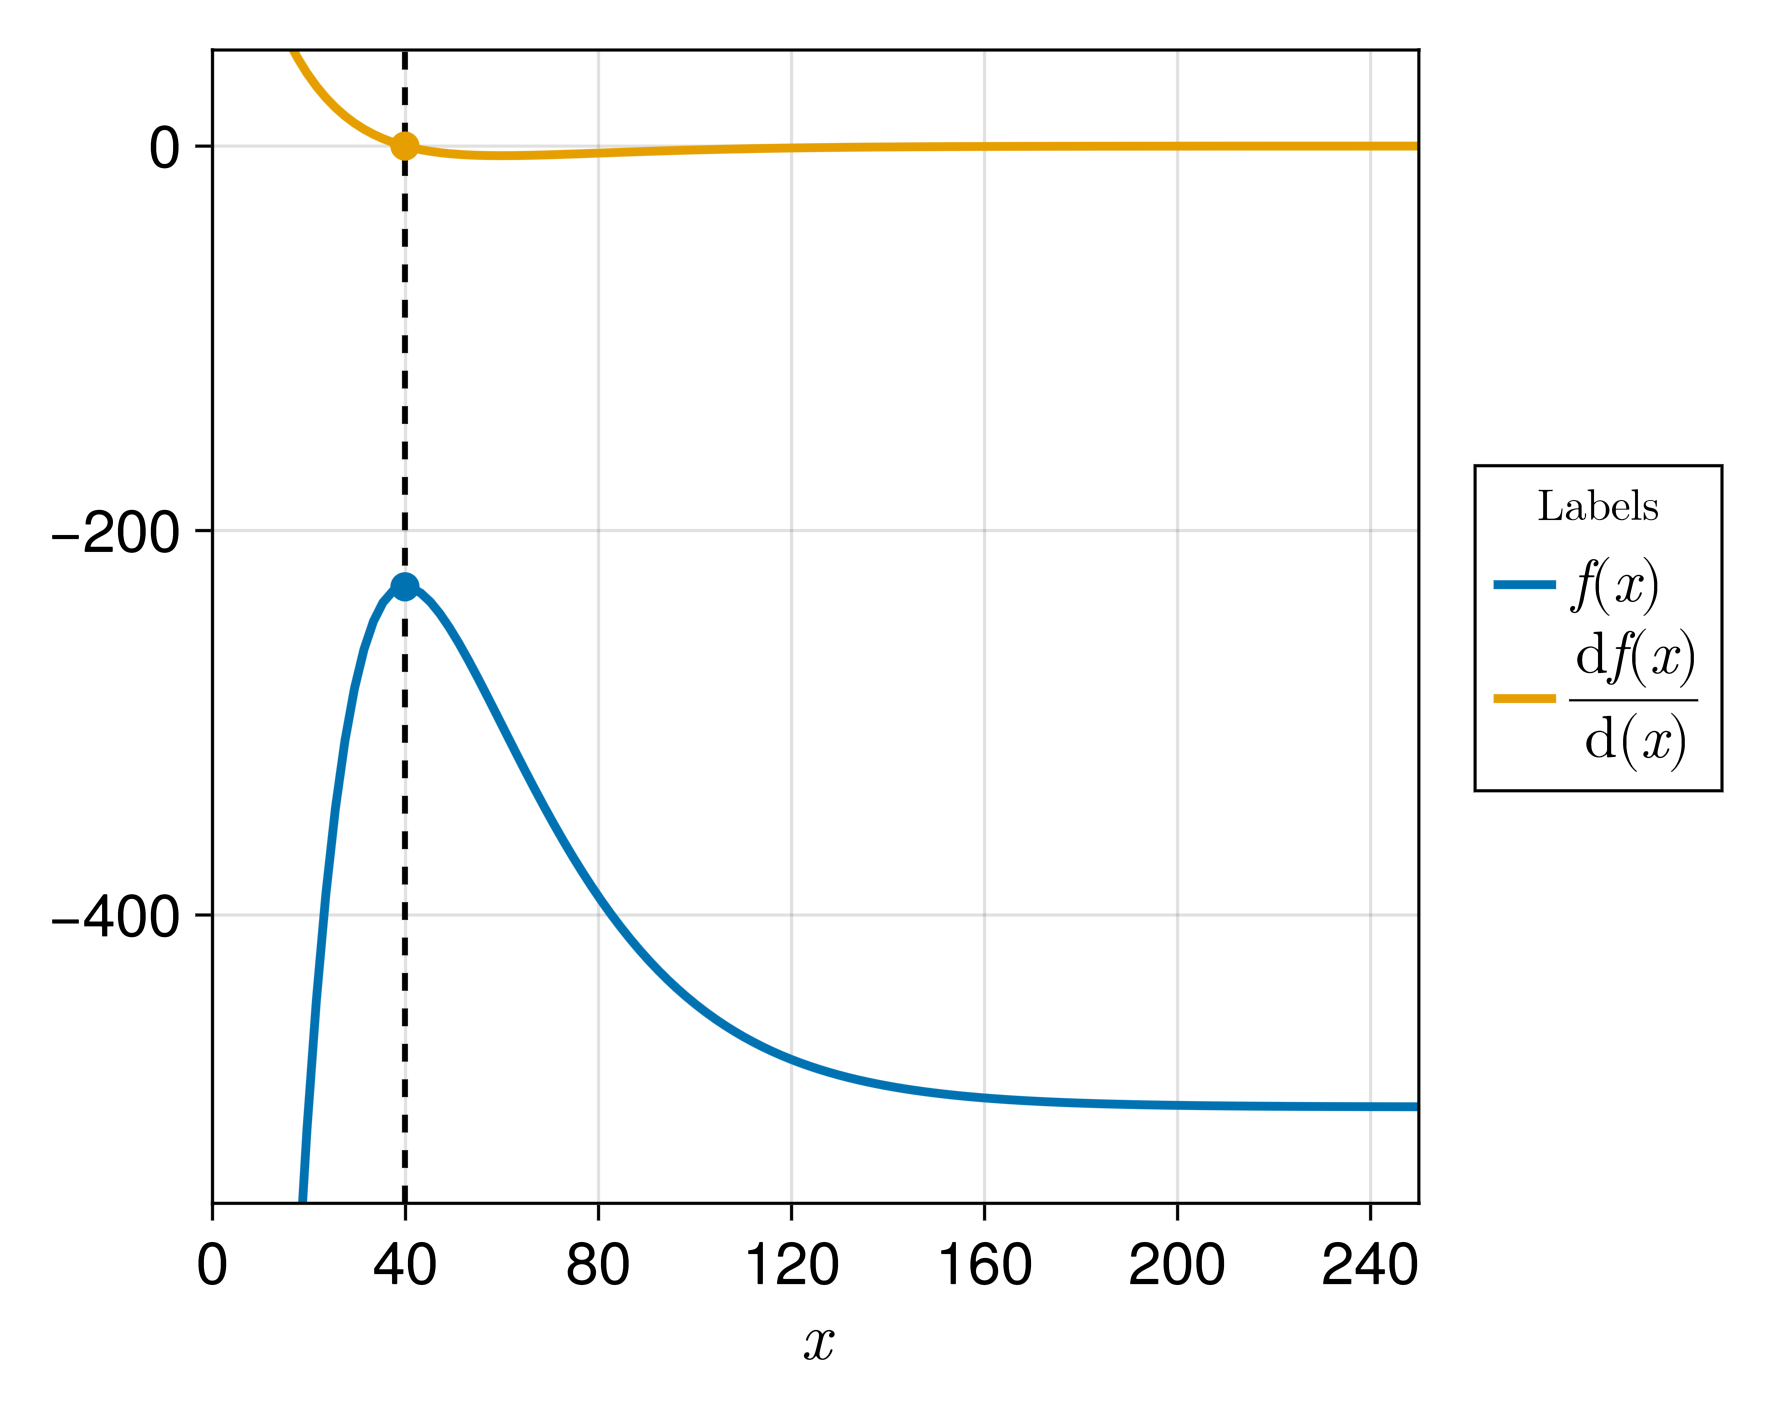
\includegraphics[width=0.45\textwidth]{../Figures/fig_exampleCrPnt2.png}
\end{figure}



\end{frame}


\end{document}
